%\documentclass[]{report}
%\usepackage[ngerman]{babel}
%\usepackage{hyphenat}
%\hyphenation{Mathe-matik wieder-gewinnen}



% Title Page
%\title{Ingenieurmäßige Arbeit}
%\author{Eshan Savla}


%\begin{document}
%\maketitle

%\begin{abstract}
%\end{abstract}

%\tableofcontents
%\vspace{2cm}

%\chapter{Einleitung}
%Industrieroboter werden primär in der Industrie für die Aufgabe der Handhabung, Montage oder Verarbeitung von Werkstücken und Teile eingesetzt. Häufig finden Industrieroboter als Schweißroboter, Lackierroboter oder Montageroboter Anwendung. Diese Art der Roboter sind meistens nicht autonom und müssen bei Bedarf für ihre Aufgabenausführung an neuen Produkte oder Werkstücke angepasst und umprogrammiert werden.


%\end{document}          


\documentclass[
	fontsize=11pt, 		% Schriftgröße
	BCOR=8mm,			% Bindekorrektur (wird nicht benötigt, da Seitenrand definiert ist)
	DIV=calc,			% Satzspiegel automatisch berechnen
	ngerman, 			% für Umlaute, Silbentrennung etc.
	a4paper, 			% Papierformat
	oneside, 			% zweiseitiges Dokument (oneside - einseitig, z. B. für Bachelor-,Studien-, oder Masterarbeit)
	titlepage, 			% es wird eine Titelseite verwendet
	parskip=half, 		% Abstand zwischen Absätzen (halbe Zeile)
	headings=normal, 	% Größe der Überschriften verkleinern
	listof=totoc, 		% Verzeichnisse im Inhaltsverzeichnis aufführen
	bibliography=totoc, % Literaturverzeichnis im Inhaltsverzeichnis aufführen
	index=totoc, 		% Index im Inhaltsverzeichnis aufführen
	final, 				% Status des Dokuments (final/draft)
	numbers=noenddot,	% keine abschließenden Punkte bei Kapitelzahlen
	footheight=30pt,	% Höhe des Raumes für Fußnoten
	headheight=30pt,]{scrbook}
% PDF-einbinden ----------------------------------------------------------------
\usepackage{pdfpages} % FH-Dortmund Logo
\usepackage[ngerman]{babel} % für deutsche Sprache
\usepackage{csquotes} %Anführungszeichen
\usepackage[backend=biber,style=authoryear,sorting=nyt,autocite=inline, maxnames=2, minnames=2]{biblatex}%Literaturverzeichnis
\usepackage{amsmath} % matritzen
\usepackage{tabularx} % mehrzeilige Tabelle
\usepackage[a4paper]{geometry} %Seitengeometrie
\usepackage{changepage} %ändert Seiten Einstellung
\usepackage{lipsum}
\usepackage{lscape} %Querformat
\usepackage{acronym} % Abkürzungsverzeichnis
\usepackage{amssymb} % Symobl reelle Zahlen
\usepackage{placeins} %behalte Bilder in der zugehörigen Section
\usepackage{makecell} % Zeilenumbruch in Tabelle
\renewcommand{\cellalign}{tl}
\usepackage[T1]{fontenc}% wichtig für Trennung von Wörtern mit Umlauten
\usepackage{microtype}% verbesserter Randausgleich
\usepackage{booktabs} % schönere Tabellen
\usepackage{caption} % Bild aus Abbildungsverzeichnis entfernen
\usepackage{subcaption}
\usepackage{lmodern}
\usepackage{graphicx}
\usepackage{blindtext}
\usepackage{siunitx}
\usepackage{float}
\usepackage{listings}
\usepackage{xcolor}
%\usepackage{abstract}
%\usepackage[authoryear]{natbib}
% Meta-Informationen -----------------------------------------------------------
%   Definition von globalen Parametern, die im gesamten Dokument verwendet
%   werden können (z.B auf der Titelseite etc.).
%          
% ------------------------------------------------------------------------------
\newcommand{\iatitle}{Die intelligente Schweißrobotik}
\newcommand{\engltitle}{Intelligent welding robots}
\newcommand{\beschreibung}{Eine Untersuchung der Anforderungen und Funktionsweise eines autonomen Schweißroboters}
\newcommand{\autor}{Eshan Savla}
\newcommand{\Matrikelnr}{7203288}
\newcommand{\Erstpruefer}{Prof. Dr.-Ing. Dennis Ziegler}
\newcommand{\Zweitpruefer}{Max Daiber-Huppert, M.Sc.}
%\bibliography{Literatur/Quellen.bib}
\addbibresource{Literatur/Quellen.bib}
\DefineBibliographyStrings{german}{andothers = {et al.}}
\setlength\bibitemsep{1.5\itemsep}  % Spacing between bib entries

\hypersetup{
	pdftitle={Bachelorarbeit-Savla},
	pdfauthor={Eshan Savla},
	colorlinks=false,
	}

\algrenewcommand\textproc{}% Used to be \textsc

%%colour and style settings code blocks
%\definecolor{codegreen}{rgb}{0,0.6,0}
%\definecolor{codeteal}{rgb}{0,0.5,0.5}
%\definecolor{codeyellow}{rgb}{0,1,1}
%\definecolor{codedandelion}{rgb}{1,0.84,0.4}
%\definecolor{codepurple}{rgb}{0.79,0.17,0.57}
%\definecolor{codeblue}{blue}{0,0.43,0.72}
%
%\lstset{emph={%
%		class, def%
%	 	}
%}
%
%\lstdefinestyle{pythonstyle}{
%	commentstyle=\color{codegreen},
%	keywordstyle=\color{codeblue},
%	stringstyle=\color{color}
%	
%}
\geometry{paper=a4paper,left=30mm,right=20mm,top=30mm,bottom=30mm}
\onehalfspacing
\RedeclareSectionCommand[afterindent=false,beforeskip=-\topskip]{chapter}

%Worttrennung
\babelprovide[hyphenrules=ngerman-x-latest]{ngerman}
\hyphenation{Nach-bar-punkte fälsch-lich-er-weise falsch-mark-ierten Stand-ard-ab-weichung vor-ge-filterte Proto-typen-phase Exakti-fizierung Kanten-erkennung Kanten-segmentierung Pro-gramm-ier-schnitt-stelle Winkel-abstand Winkel-abstände Winkel-abstands Rand-punkten Rand-punkt Rand-punkte Hard-ware-beschleunigung Punkte-abstand Punkte-abstände Punkt-abständen}

\begin{document}
	\begin{titlepage}
% Titelseite ohne Seitenzahl
\vspace{2cm}

\begin{center}
\large\textbf{Fachhochschule Dortmund \\}
\vspace{2cm}
\large{Fachbereich: Maschinenbau \\}
\large{Studiengang: Maschinenbau (B.Eng.)}
\vspace{2cm}

\includegraphics[width=10cm]{"Abbildungen/FH_Dortmund-logo".png}  %Logo der FH einfügen
\vspace{1cm}

\large{\textbf{\iatitle}}\\
\vspace{0.5cm}
\large{\beschreibung}

\vspace{1.5cm}

\begin{tabular}{ll}
Erstprüfer: & \Erstpruefer \\
Zweitprüfer: & \Zweitpruefer \\
\end{tabular}

\vspace{1.5cm} 

\large{Vorgelegt von\\
\textbf{\autor}\\
Matrikelnummer: \Matrikelnr\\
am \today}
\end{center}
\end{titlepage}
	\pagenumbering{Roman}
	\setcounter{page}{2}
	%\chapter*{Eidesstattliche Erklärung}

Hiermit erkläre ich, dass ich die vorliegende Arbeit eigenständig und ohne fremde Hilfe angefertigt habe. Textpassagen, die wörtlich oder dem Sinn nach auf Publikationen oder Vorträgen anderer Autoren beruhen, sind als solche kenntlich gemacht. Die Arbeit wurde bisher keiner anderen Prüfungsbehörde vorgelegt und auch noch nicht veröffentlicht.
\vspace{0.5cm}

Stuttgart, \today

\vspace{0.5cm}

\_\_\_\_\_\_\_\_\_\_\_\_\_\_\_\_

Eshan Savla


%	\section*{\centering Zusammenfassung}
Die Erkennung von geometrischen Merkmalen eines Objektes, während es durch einen optischen Sensor abgetastet wird, hat für die sensor-basierte Programmierung von Robotern eine hohe Relevanz. In dieser Arbeit wird ein numerisches Verfahren für diesen Zweck vorgestellt. Das Ziel dieser Arbeit ist die Bewertung der Effektivität des Verfahrens. Dazu ergänzend wird diese Forschungsfrage gestellt: Wie Effektiv ist ein numerisches Verfahren bei der Kantenerkennung und Segmentierung von wachsenden Punktwolken? Zuerst wurde das AGPN-Verfahren aus der Literatur reproduziert sowie für den Einsatzzweck angepasst und erweitert. In dieser Arbeit werden die Schritte zur Erweiterung des Verfahrens detailliert beschrieben sowie auf Methoden zur Entfernung falsch-detektierten Kanten eingegangen. Zur Beantwortung der Forschungsfrage wurden drei Untersuchungen konzipiert. Konkret wurde die Genauigkeit und Robustheit des Verfahrens unter verschiedenen Bedingungen überprüft und auf Basis der erkannten und segmentierten Kanten bewertet. Auch der Einfluss einer absteigenden Punktdichte auf die Genauigkeit wurde im Rahmen der Arbeit überprüft. Zu diesen Tests werden synthetische Dateien sowie reelle Aufnahmen von Bauteilen präsentiert. Diese Arbeit lieferte das Ergebnis, dass das Verfahren zu einer hohen Genauigkeit und Robustheit gegen Rauschen Kanten von geometrischen Merkmalen erkennen und segmentieren kann. Daneben wurden auch wichtige Erkenntnisse über die Schwachstellen und Grenzen des Verfahrens gewonnen. Schließlich werden aufbauende Forschungsmöglichkeiten im Bereich der Robotik und Automatisierung besprochen.

\section*{\centering Abstract}
The recognition of geometric features of an object while being scanned by an optical sensor is of high relevance for sensor-based robotics programming. This paper presents a numerical method for this purpose and aims to evaluate its effectiveness. The research question posed pertaining to this aim is: How effective is a numerical method for edge detection and segmentation in growing point clouds? Initially, the AGPN Method from current literature was reproduced before being adapted and extended with additional functionalities to make it suitable for the specific application case. The steps taken to extend the method are detailed in this paper, including methods for removing falsely detected edges. Three studies were designed to answer the research question, where the accuracy and robustness of the method was tested under different conditions and evaluated based on the number of accurately detected and segmented edges. Besides testing the accuracy of the method, effects of decreasing point density were also studied. This paper presents a controlled ground truth as well as a variety of scans of real objects used in these tests. The result showed that the method can detect and segment edges of geometric features with high accuracy, while also resisting high amounts of noise. Finally, weaknesses, limitations and future research opportunities on the basis of this method in the field of robotics and automation are discussed.

	\newpage
%\setuptoc{toc}{totoc} %Inhaltsverzeichnis im Inhaltsverzeichnis
\tableofcontents
\newpage
\addchap{Abkürzungsverzeichnis}
%Führe lieber keine Abkürzungen ein, wenn du sie nicht mindestens dreimal verwendest. Das gilt allerdings nicht für Fachausdrücke, die standardmäßig abgekürzt werden.

%Deine nicht allgemein gebräuchlichen Abkürzungen solltest du im Abkürzungsverzeichnis einführen.
\begin{acronym}[Grundlagen]
\acro{agpn}[AGPN]{Analysis of Geometric Properties of Neighbourhoods}
\acro{iefd}[IEFD]{Iterative Edge and Feature Detection}
\acro{ransac}[RANSAC]{Random Sample Consensus}
\acro{pcl}[PCL]{Point Cloud Library}
\acro{ros}[ROS]{Robot Operating System}
\end{acronym}
\newpage
\listoffigures
\listoftables
	
	\pagenumbering{arabic}
	\chapter{Einführung in der intelligenten Robotik}
\section{Robotik in der Industrie} \label{sec:Industrieroboter}
Industrieroboter werden primär in der Industrie für die Aufgabe der Handhabung, Montage oder Verarbeitung von Werkstücken und Teile eingesetzt. Häufig finden Industrieroboter als Schweißroboter, Lackierroboter oder Montageroboter Anwendung. Diese Art der Roboter ermöglichen in diesem Umfeld eine günstigere, genauere und zuverlässigere Verarbeitung von Produkten und Werkstücken. \autocite{maier2016grundlagen}

Industrierobotern fanden ihre erste Anwendung in der 1960er Jahren in der Automobilindustrie in den USA. Durch die Einführung von japanischen Industrierobotern in den 1980er Jahren erlebten japanischen Unternehmen zur Folge von Lean-Product¸ion und Kaizen-Konzepten eine erhebliche Steigerung ihrer Produktivität und Qualität. Unter Konkurrenzdruck  forderten europäischen und nordamerikanischen Automobilehesteller leistungsstärkerer und bessere Industrieroboter an und setzten diese ein. Seitdem entsteht die Nachfrage für Industrieroboter hauptsächlich von großen Unternehmen. Im Jahr 2008 entstand 70\% dieser Nachfrage aus der Automobilindustrie.\autocite{Bierfreund+2008+135+140}

Von den Vorteilen der Automatisierung und Robotik in einem industriellen Umfeld können nicht nur großen Unternehmen profitieren, sondern auch kleinen und mittelständischen Unternehmen. Die Robotik bringt insbesondere den Firmen einen Vorteil, die in einem Arbeitsmarkt agieren, wo qualifizierte und ausgebildete Arbeitnehmer eine Mangelware sind und Arbeitskosten allgemein hoch oder sehr hoch sind. Durch den Einsatz von Industrierobotern in der Produktion könnte dieser Mangel an ausgebildeten Arbeitskräften ausgeglichen werden. 80\% der, durch Personalkosten entstehenden Prozesskosten des Schweißens in der Produktion, können mittels Industrieroboter abgeschafft werden. \autocite{glaser2008industrial}

Für den Einsatz in kleinen und mittelständischen Unternehmen müssen Industrieroboter gewisse Anforderungen dieser Unternehmen erfüllen. Um die Ansprüche auf kleineren Losgrößen und der Einzelfertigung kleiner und mittelständiger Unternehmen erfüllen zu können, müssen Robotersysteme nicht nur mit unterschiedlichen Werkstückgeometrien zurechtkommen, sondern diverse Aufgaben ausführen können. Ein häufiges Programm- und Werkzeugwechsel des Roboters ohne die Voraussetzung von Expertenwissen soll bei dieser neuen Generation von Robotersysteme ein Standard werden. \autocite{Bierfreund+2008+135+140}

Obwohl die Technik der Industrieroboter seit den letzten Jahren rasant weiterentwickelt wurde, sind diese Art der Roboter  meistens nicht autonom. Sie müssen bei Bedarf für ihre Aufgabenausführung an neuen Produkte oder Werkstücke angepasst und umprogrammiert werden. \autocite{maier2016grundlagen}. Eine schnelle Anpassung oder Umprogrammierung des Roboters ist ein wesentliches Kriterium für die Erreichung eines hohen Flexibilitätsgrades. Diese Erhöhung der Flexibilität ist durch die Errichtung von \emph{intelligenten} Prozessen möglich, die mit der Verwendung von Sensoren und Reglungen den herkömmlichen Prozessen gegenüber eine Verbesserung darstellen. Roboter wandeln somit von normalen Handhabungsgeräten zu cyberphysische Systeme, die ihre Umgebung wahrnehmen können und sich somit auf Störungen oder Änderungen anpassen können. \autocite{MeyerChristian2007RaSd}
\autocite{HägeleMartinFraunhoferIPA2016SfdP}

Auch für die sichere Mensch-Roboter-Kollaboration sind sensor-ausgerüstete Roboter nicht nur vorteilhaft, sondern auch nötig, insbesondere für kleine und mittelständische Unternehmen. Mit kollaborierenden Robotern können auf teure Sicherheitseinrichtungen verzichtet werden, welches für diese Unternehmen eine große Ersparnis anbietet. Eine Entwicklung der Fraunhofer Institut für Produktions- und Automatisierungstechnik (IPA) - ein kognitiver Schweißroboter - ist ein Beispiel eines, durch Sensorik und Robotik verbesserten Produktionsprozesses. Die Lokalisierung des Produktes mit einer Genauigkeit von unter einem Fünftel Millimeter erfolgt durch die Verwendung von 3D-Sensordaten. Vorteile davon sind eine verkürzte Einrichtungszeit und das wirtschaftliche Schweißen in kleinen Losgrößen, da es keine komplizierten Fixierungen benötigt werden. \autocite{HägeleMartinFraunhoferIPA2016SfdP}

\section{Motivation} \label{sec:motivation}
Es gibt in der Industrierobotik einige Durchbrüche, die zu der Weiterentwickelung von intelligenten Robotern geführt haben. Industrieroboter wurden hinsichtlich ihrer Flexibilität, Genauigkeit, Einsatzmöglichkeit und Kollaboration mit Menschen verbessert.

Die Arbeit von \textcite{Liu2022} umfasst die Mitbetrachtung der Umwelt und dynamischer externer Störungen bei der Bahnplanung von Robotern. Es wird über die Überlagerung der statischen oder offline Planung mit einer dynamischen oder online Planung diskutiert. Die offline Planung umfasst die Navigation eines Roboters unter Betrachtung aller globalen Elemente. Demgegenüber handelt es sich bei der online Planung um die Anpassung der vorgeplanten Bahn des Roboters auf Basis der Umgebungsänderungen in Echtzeit. Durch die Verwendung maschinellen Sehens haben die Autoren Methoden zur Erkennung dynamischer Änderungen der Umwelt entwickelt, sodass Roboter beispielsweise spontan erschienene Hindernisse auf der Bahn erkennen und vermeiden können. 

\textcite{Luo2016} haben Roboter in cyber-physischen Systemen durch die Implementierung von IoT Methoden umgewandelt. Es wurden Aktoren und Sensoren mit einander vernetzt, um einen Informationsaustausch für die Erledigung Produktionsaufgaben zu ermöglichen. Dabei wurden Methoden basiert auf maschinellem Sehen für Aufgaben wie Objekterkennung, Greifen von Objekten, Hindernisvermeidung und Sicherheitsgewährleistung vorgeschlagen und entwickelt. 

\textcite{Wang2012} schlagen einen Plan für multiple kollaborierende Roboter die mit einander vernetzt sind und kommunizieren können. Information aus dem Sensor eines Roboters steht anderen beteiligten Robotern des Netzwerks zur Verfügung. Beispielsweise sind diese vernetzten Roboter über die aktuellen Positionen anderer Roboter bewusst. Mit der Anwendung von Methoden aus dem maschinellem Lernen sind diese Schwarmroboter in der Lage, komplexe logistische Probleme zu lösen.

Über die Zeit sind verschiedene Projekte entstanden, die ein autonomes Handeln für Roboter entwickelt haben, das einen flexibleren Einsatz dieser Roboter in dynamischen Produktionssysteme ermöglichen sowie mehr Menschen-Roboter-Kollaboration fördern. Diese Projekte werden auch überall in der Welt gefördert, da steigender Lohnkosten und ein steigendes Durchschnittsalter in vielen Ländern ein drohendes Problem darstellt. \autocite{Wang2018} \autocite{Marguglio2022}

Die Fraunhofer Institut für Produktions- und Automatisierungstechnik entwickelt einen intelligenten kollaborierenden Roboter, einen Cobot, um das automatisierte Schweißen für kleinere Losgrößen zu realisieren. Es soll die Programmierung eines solchen Roboters für die Industrieanwendung vereinfacht werden, sodass trotz mangelnden Expertenwissens und eines Fachkräftemangels kleinere Betriebe von erhöhten Produktionsfähigkeiten gewinnen können. Dabei sind die Investitionskosten eines Cobots deutlich geringer sowie verfallen die Installationskosten, da keine Sicherheitsvorkehrungen bei Cobots notwendig sind. \autocite{automationspraxis_2021} 

Die Programmierung bestehender Cobots mit dem Teach-In-Verfahren ist zwar einfach, allerdings ist sie auch sehr zeitintensiv. Eine Programmierung auf Basis CAD-Daten eines Bauteils ist nicht immer möglich, da diese Daten manchmal bei kleinen und mittelständischen Unternehmen nicht vorhanden sind. Mittels eines Laserliniensensors wird die Programmierung und Trajektorienplanung des Roboters einfacher und effizienter gemacht. Der Sensor erkennt optisch die Kehlnaht und ihrer Position in Echtzeit und benutzt diese Information zur Steuerung der Roboterbewegung. Der Anwender muss dem Roboter und den Schweißbrenner grob über den Werkstück positionieren, danach den Start- und Endpunkt festlegen. Nach dem Programmstart erkennt der Roboter die Kehlnaht und positioniert den Schweißbrenner genau auf sie hin. Danach wird der Kehlnaht entlang geschweißt sowie Änderungen in der Naht-Geometrie erkennt und die Trajektorie angepasst. \autocite{automationspraxis_2021}

Das Ziel dieser Arbeit ist es, den kollaborierenden Schweißroboter der Fraunhofer IPA und seine Funktionsweise zu untersuchen. Dabei sollen die einzelnen Hardware- und Softwarekomponenten genauer betrachtet werden. Es soll die Frage beantwortet werden: Welche Hardware- und Softwareanforderungen gibt es für die automatische Schweißnaht-Erkennung durch ein intelligentes kollaborierendes Robotersystem.

\section{Struktur dieser Arbeit}
Im folgenden wird die Aufbau dieser Arbeit und die einzelnen Inhaltsteile kurzgefasst. Nach der obigen Zielsetzung dieser Arbeit werden theoretische Grundlagen zur Verständnis der Funktionsweise diskutiert. Danach folgt eine detaillierte Beschreibung der aktuellen Technik und Funktionsweise des Schweißroboters. Schließlich werden die wesentlichen Erkenntnisse dieser Arbeit zusammengefasst und präsentiert.

Es wird in den Grundlagen der Robotermechanik und -Kinematik eingetaucht. Hier wird der Grundaufbau eines Industrieroboters zusammen mit der Funktion seiner Einzelteile vorgestellt. Beleuchtet wird auch wie die Gelenke den Arbeitsraum eines Roboters definieren und die Bewegung des Roboters beeinflussen. 

Aufbauend auf dem Thema der Industrieroboter wird das Thema der Schweißrobotik eingeführt. Neben eine Argumentation für den Einsatz von Schweißroboter in der Industrie wird über unterschiedlichen Schweißverfahren diskutiert, die häufig in der Schweißrobotik eine Anwendung finden. Es werden die Funktionsweise, benötigten Hardwareeinrichtungen und anpassbaren Parameter sowie ihren Einfluss untersucht. 

Die Sensorik findet zunehmend in der Robotik jetzt eine Anwendung. Neben anderen Sensoren zur Erkennung der Temperatur, Kraft, Haptik und Geräusch werden auch optische Sensoren als das technische Auge eines Roboters verwendet. Es werden die Grundlagen der Sensorik für die Anwendung in der Automatisierung besprochen und die Methoden zur Distanz Ermittlung diverser Lasersensoren untersucht. 

Als letztes wird das Verbindungselement der einzelnen Hardwarekomponenten vorgestellt - die Software. Hier das Robot Operating System vorgestellt, welches die Kommunikation zwischen unterschiedlichen Komponenten eines Robotersystems ermöglicht und weitere fortgeschrittene Funktionalitäten wie Simulationen, Visualisierungen, und Trajektorienplanung für Roboter anbietet.

Nach der Behandlung der Theorie wird der aktuelle technischer Stand des Roboters erläutert. Hierbei wird grundsätzlich zwischen der Hardware und Software des Robotersystems unterschieden. Es werden die Daten und Einzelfunktionen der physischen Geräte kurzgefasst. Danach wird die Software, die das autonome Roboterschweißen ermöglicht, detailliert behandelt. Hierbei wird nicht nur die Funktionsweise des Softwaremoduls abstrahiert, sondern werden die einzelnen Teilmodule betrachtet, die auf die Ausführung spezieller Teilaufgaben ausgelegt sind. Danach werden wichtige Nachrichtenprotokolle für den Austausch diverser Informationstypen wie Koordinatentransformationen oder Sensorwerte analysiert. Schließlich werden andere Softwareabhängigkeiten des Softwarepakets angeschaut, die die Softwareentwickelung für das Robotersystem erleichtern.

Schließlich werden die Erkenntnisse dieser Arbeit zusammengefasst sowie die Applikationen, Limitationen und Zukunftspotenzial des Robotersystems behandelt.
	%Datenstrukturen und Algorithmen
%	Was sind Algorithmen und Datenstrukturen
% 	Arten von Basis Datenstrukturen
%		Vector/Liste
%		Queue(Warteschlange)
%		Stack??
%		map und hash tabellen
%	besondere Datenstruktur - PCL Punktwolke
%	
%	Komplexität und Notation von Algorithmen
%	Arten von Basis Algorithmen
%		
% 		
%	besondere Algorithmen:
%		kd-tree
%		octree(vielleicht)
%		RANSAC
%		Segmentierung

\chapter{Theorie}
Im Kern dieser Arbeit steht eine Rechenaufgabe vor. Die positionellen Informationen über Objekte und Bauteile müssen sinnvoll verarbeitet werden, um die Lage und Form der geometrischen Merkmale des Objektes zu bestimmen. Bei der Entwicklung eines allgemeinen Verfahrens zur Erkennung der geometrischen Merkmale in Abschnitt~\ref{Methodik} werden Algorithmen und Datenstrukturen verwendet. 

\section{Datenstrukturen}

Datenstrukturen dienen der Organisation und Speicherung von Daten so, dass die Beziehung zwischen einzelnen Elemente auch aufbewahren wird. In einer Datenstruktur werden darüber hinaus auch Zugriffsmethoden für den Zugriff auf die gespeicherten Daten definiert sowie Angaben über Möglichkeiten zur Verarbeitung der Daten gemacht. Eine gute Datenstruktur setzt voraus, dass die Beziehung zwischen der Daten aufbewahren und gut definiert wird sowie die Verarbeitung der Daten leicht gemacht wird. Eine Datenstruktur soll auch bestimmte Operationen auf die Daten ermögliche, beispielsweise die Hinzufügung oder Entfernung von Datenpunkte, die Zusammenführung oder Sortierung der Daten sowie das Durchqueren der Datenstruktur und die Suche nach bestimmten Daten. In der Informatik gibt es bereits etablierte Datenstrukturen, die sich nach unterschiedlichen Einsatzzwecken richten und eine sehr breite Anwendung finden. Diese lassen sich nach Abbildung \ref{fig: datastructures} nach lineare und nichtlineare Datenstrukturen unterteilen. \autocite[1-2]{mohanty_data_2021}

\begin{figure}[h]
	\includegraphics[width=\textwidth]{Abbildungen/Datenstruktur_arten.png}
	\centering
	\caption{Die unterschiedlichen Arten von linearen und nichtlinearen Datenstrukturen nach \textcite[2]{mohanty_data_2021}}
	\label{fig: datastructures}
\end{figure}

\section{Algorithmen}

Ein Algorithmus ist ein Verfahren, welches zur Bestimmung einer oder mehreren Lösungen eines bestimmten Rechenproblems verwendet wird \autocite[1]{knebl_algorithmen_2021}. In einem Algorithmus wird ein Lösungsansatz möglichst präzise ausformuliert, indem kleine, isolierte und klar definierte Verarbeitungsschritte definiert werden. Auch ein simples Verfahren zur Summierung zwei Zahlen lässt sich als ein Algorithmus nennen. \autocite[9-10]{hubwieser_fundamente_2015}
	%Struktur
% -Festlegung von Software-Kriterien
% -Auswahl des Verfahrens
% -Reproduktion des Verfahrens aus der Literatur
% 	-Kantenerkennung
% 	-Segmentierung
%	-Probleme & besondere Erkenntnisse
% -Erweiterung des Verfahrens
%	-Grundlegende Änderungen des Verfahrens
%	-False edge removal
%	-Point marking and cloud filtering
%	-misc.


\chapter{Entwicklungsprozess der Software}
Die Rücksichtnahme des Einsatzzwecks bei der Design und Entwurf des Verfahrens sowie die Entwicklung der Software war erforderlich, um die gewünschte Funktionalitäten gewährleisten zu können. Das Verfahren soll Kanten und Geometrien nicht nur in vollständig generierten Punktwolken erkennen, sondern auch in unvollständige Punktwolken, die iterativ wachsen. Hierbei wird ein Laserliniensensor eine Kante eines Werkstücks oder Objektes entlang geführt und somit sequentiell abgetastet. Deswegen wird die räumliche Struktur des Objektes nicht in einer einzigen Aufnahme abgebildet, sondern durch mehrere kleine Einzelaufnahmen. Der intelligente Schweißroboter, der durch das Fraunhofer Institut für Produktions- und Automatisierungstechnik entwickelt wird, verwendet ein solches Verfahren zum Scannen eines Werkstückes und zur Erkennung Schweißnähte \autocite[39]{savla_intelligente_2022}. Mittels eines Lasersensors wird die Oberfläche des Werkstückes dreidimensional abgebildet. Aktuell wird eine Schweißkegelnaht durch die Erkennung der Schnittlinie zwei Ebenen markiert, die mittels RANSAC-Algorithmen auf die Punktwolke des Werkstückes gefittet werden. Dieses Verfahren zur Erkennung der Schweißnaht bietet allerdings kaum detaillierte Informationen über die Geometrie des Werkstückes an.\autocite[39-52]{savla_intelligente_2022}. Das, in dieser Arbeit entwickelte Verfahren soll das bestehende Verfahren ersetzen und somit seine Limitationen überwinden.

\begin{figure}[h]
	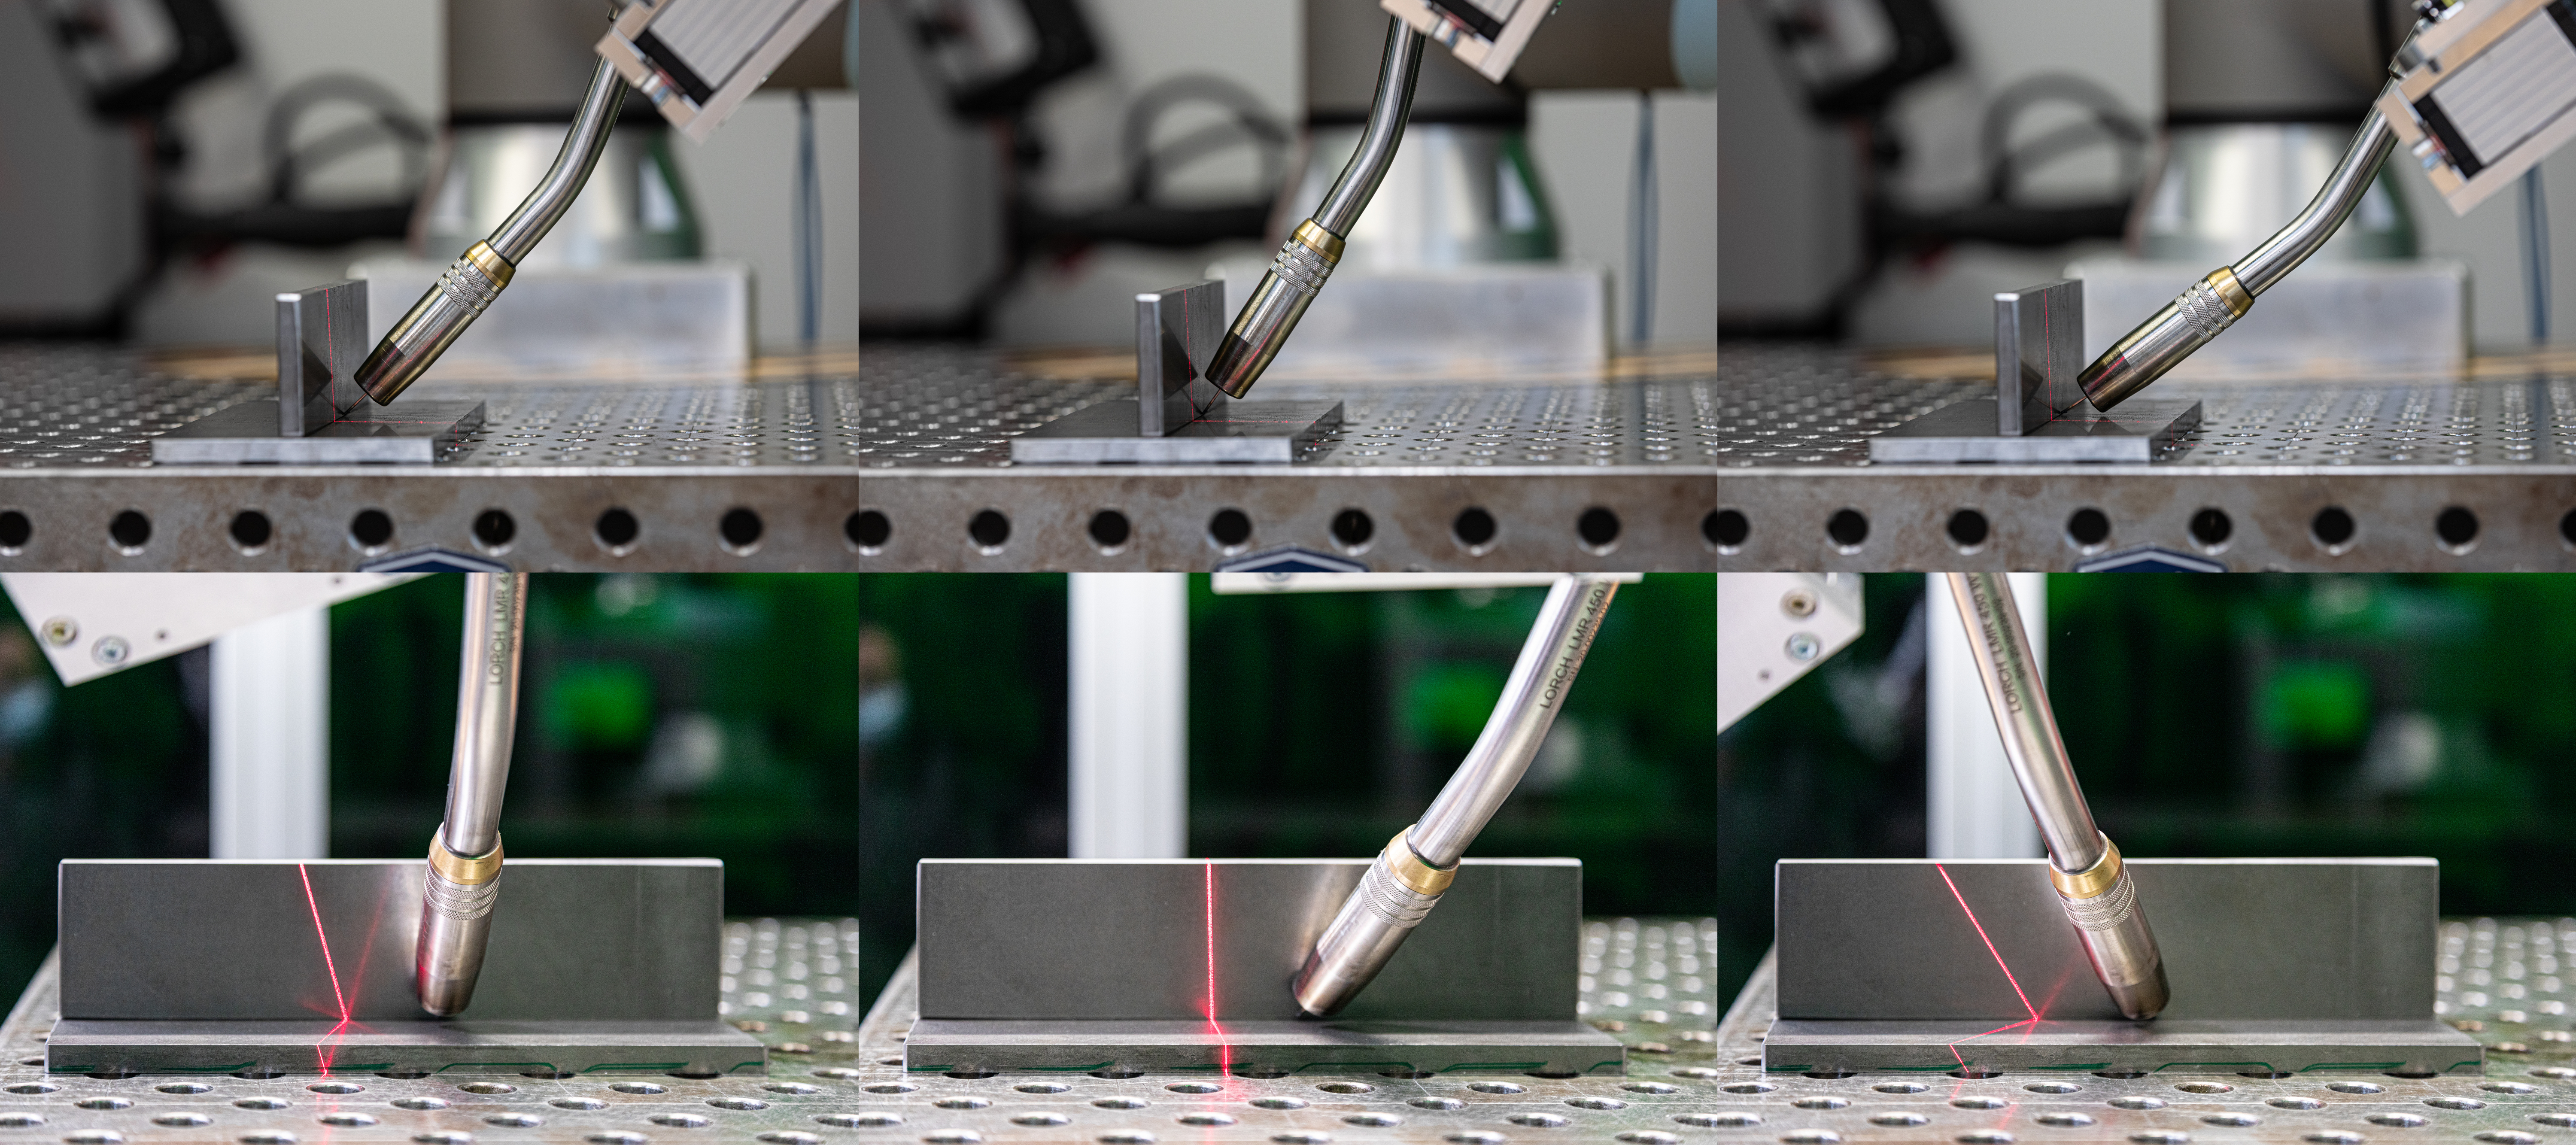
\includegraphics[width = \textwidth]{Abbildungen/collage.jpg}
	\centering
	\caption{Der Laserliniensensor} 
\end{figure}

\section{Vorbereitungen}
\subsection{Software-Voraussetzungen}\label{soft_voraus}
Bei der Auswahl eines geeigneten Verfahrens zur Detektierung Kanten in einer Punktwolke wurden einige Voraussetzungen festgelegt. Die Methode sollte in der Lage sein, nicht nur Außenkanten zu erkennen, sondern auch Innenkanten beziehungsweise Faltungen. Neben dem originellen Einsatzzweck sollte das Verfahren möglichst breit anwendbar sein und eine hohe Modularität aufweisen. Die Funktionen der Kantendetektierung und Punktesegmentierung sollten unabhängig von einander aufrufbar gestaltet werden, um dem Benutzer eine möglichst hohe Flexibilität anzubieten. Die Kantenerkennung sollte performant erfolgen und Punktwolken innerhalb eines praktischen Zeitraums verarbeiten. Letztlich soll das Programm in dem bestehenden Programmpaket des Schweißroboters integrierbar sein. Die Hardwarebeschleunigung des Verfahrens mittels eines Grafikprozessors wurde ausgeschlossen, da ihrer Verwendung mit dem Echtzeitkernels des Programmpakets zur Konflikte führt. 

\subsection{Auswahl eines Verfahrens}
Eine Literatursuche nach Verfahren zur adaptiven Erkennung von Kanten in wachsenden 3D Punktwolken für den Einsatzzweck ergab nichts. Die meisten Verfahren eigneten sich für die Kantenerkennung nur in vollständigen Punktwolken. Aus diesem Grund wurde die Entscheidung getroffen, ein vorhandenes Verfahren aus der Literatur zu wählen und es für den Einsatzzweck anzupassen. Drei unterschiedlichen Verfahren nach \textcite{bazazian_edc-net_2021}, \textcite{himeur_pcednet_2021} und \textcite{rachmadi_road_2017} zeigten viel versprechende Ergebnisse. Allerdings wurden neuronale Netze in dieser Verfahren verwendet, welches zu zwei Problemen geführt hätte. Aufgrund der Funktionsweise neuronaler Netze wäre es schwierig gewesen, diese für den Einsatzzweck ohne eine umständliche Anpassung des neuronalen Netzes anzupassen. Das zweite Hindernis entsteht durch die Einschränkung bei der Verwendung von Grafikprozessoren. Diese Prozessoren hätten die Rechenzeit neuronaler Netze sehr stark verringert und die schnelle Performanz des Verfahrens gewährleistet \autocite[625]{luo_artificial_2005}. Das numerische Verfahren nach \textcite{choi_rgb-d_2013} war auch für den Einsatzzweck ungeeignet, da es als Eingangsparameter eine RGB-D Datei erfordert. Somit wäre das Verfahren nur für eine Anwendung auf organisierten, gefärbten Punktwolken eingeschränkt. Es wurden zwei weitere Verfahren gefunden, die sich zur Erkennung Kanten in organisierten sowie unorganisierten Punktwolken eignen würden. \textcite{mineo_novel_2019} stellten eine numerische Methoden vor, welche zu einer hohen Genauigkeit Kanten erkennen konnte. Allerdings wurden keine Angaben über die Erkennung Innenkanten in dieser Arbeit gemacht. \textcite{ni_edge_2016} schlagen im Gegensatz eine Methode namens AGPN vor, die nicht nur Außen- sowie Innenkanten und Faltungen erkennt, sondern die erkannten Randpunkte zusammen clustert, um Kannten voneinander zu trennen. Diese Studie präsentierte ein Verfahren mit einer hohen Genauigkeit sowie eine Möglichkeit, die Randpunkte sinnvoll zusammen zu gruppieren. Aus diesem Grund wurde dieses Verfahren als Grundlage für das adaptive Verfahren dieser Arbeit gewählt.

\section{Reproduktion des AGPNs}
Bevor das Verfahren für den Einsatzzweck angepasst wurde, wurde es zuerst zwecks einer Überprüfung unverändert implementiert. Es sollte sichergestellt werden, dass das Verfahren für die Erkennung Innenkanten und potenzielle Schweißnähte geeignet ist. Da die Autoren das Quellcode ihres Verfahrens nicht öffentlich zugängig gemacht haben, musste das Programm händisch reproduziert werden. Die Reproduktion des Programms erfolgte in zwei Schritten - die Reproduktion des Verfahrens zur Kantenerkennung und dessen zur Kantensegmentierung. Obwohl andere Skriptsprachen wie Python und MATLAB hinsichtlich des Prototypings Vorteile anbieten, wurde das Programm in C++ wegen seiner besseren Leistungsfähigkeit implementiert \autocite{svensson_performance_2021}. Viele Funktionalitäten der PCL-Bibliothek \autocite{rusu_3d_2011} wurden auch zum Entwurf des Verfahrens verwendet.

\subsection{Verfahren zur Erkennung Randpunkte}
Während Randelemente in zweidimensionale Bilder als eine klare Definition haben, fehlt eine solche Definition für Randelemente und Kanten in 3D-Punktwolken. In diesem Verfahren wurden die geometrischen Eigenschaften einer Kollektion von Punkten zur Erkennung Randpunkte berücksichtigt. Randpunkte weisen eine besondere geometrische Eigenschaft auf - der Winkelabstand zwischen benachbarten Randpunkte ist im Vergleich zu anderen benachbarten Punkten deutlich größer. Faltungen stellen den Grenzbereich zwischen zwei angrenzenden Ebenen dar, deren Normale in unterschiedlichen Richtungen zeigen. Diese geometrischen Eigenschaften wurden zur Erkennung Randpunkte verwendet. \autocite[1-2]{ni_edge_2016}

\begin{figure}[h]
	\includegraphics[scale=0.12]{Abbildungen/ablauf_plan_edge.png}
	\centering
	\caption{Das Programmablaufplan zur Erkennung Randpunkte \autocite{ni_edge_2016}.}
	\label{flow_chart}
\end{figure}

Im folgenden wird das Verfahren zur Erkennung Randpunkte detaillierter erläutert. Für einen Punkt \textit{o} wurde eine Sammlung von \textit{K\textsubscript{1}} benachbarten Punkten mittels eines kd-trees erstellt. Diese Sammlung wird als eine Nachbarschaft \textit{N\textsubscript{o}} referiert. Danach wurde mittels eines RANSAC-Algorithmus eine Ebene \textit{E\textsubscript{N}} auf diese Nachbarschaft gefittet, um Ausreißer herauszufiltern und zwei angrenzenden Flächen innerhalb der Nachbarschaft voneinander zu trennen. Danach wurde Überprüft, ober der Punkt \textit{o} auf der RANSAC-Ebene lag. Falls dieser Punkt ein Ausreißer der Ebene \textit{E\textsubscript{N}} war, wurde er nicht als einen Randpunkt markiert. Ansonsten wurden weiterhin die geometrischen Eigenschaften der Nachbarschaft überprüft. Abbildung \ref{RANSAC-Ebene} visualisiert die Trennung zwischen unterschiedlichen Flächen einer Punktwolke mittels des RANSAC-Verfahrens. 

\begin{figure}[h]
	\includegraphics[width=\textwidth]{Abbildungen/RANSAC-Ebene.png}
	\centering
	\caption{Eine lokale RANSAC-Ebene (rot dargestellt) neben anderen Oberflächen (blau dargestellt). In \textbf{a} sind drei Ebenen zu sehen, wobei in \textbf{b} nur zwei zu sehen sind. \autocite{ni_edge_2016}}
	\label{RANSAC-Ebene}
\end{figure} 

Im Falle, dass der Punkt \textit{o} ein Inlier war und zu der Ebene \textit{E\textsubscript{N\textsubscript{o}}} gehörte, fang die tatsächliche Überprüfung der geometrischen Eigenschaften der Nachbarschaft \textit{N\textsubscript{o}} an. Um die Ebenengleichung von \textit{E\textsubscript{N}} näherungsweise zu schätzen, wurde zuerst die Normale \textit{$\vec{n}$} der Ebene geschätzt. In einer effizienten Weise wurde die Ebenengleichung durch das RANSAC-Verfahren näherungsweise geschätzt. Diese Gleichung wurde weiterhin auf die RANSAC-Inliers optimiert und daraus die Normale \textit{$\vec{n}$} ermittelt. Danach erfolgte die Errechnung des Winkelabstands zwischen den jeweiligen Punkten von \textit{N\textsubscript{o}}. Hierfür wurden für die Ebene \textit{E\textsubscript{N}} die jeweiligen Eigenvektoren $\vec{u}$ und $\vec{v}$ aus der Normale $\vec{n}$ errechnet. Das fertige Verfahren von PCL zur Ausrechnung der Eigenvektoren lieferte ungenaue Ergebnisse. Stattdessen wurden zur Ermittelung \textit{$\vec{u}$} zwei zufällig gewählte Punkten aus der Inliers verwendet. Es wurde dabei sichergestellt, dass keiner der Punkten den Punkt \textit{o} entsprachen. Zur Errechnung des Winkelabstands wurden zuerst die Winkel aller Punkte der lokalen Ebene \textit{E\textsubscript{N}} errechnet. Mit dem Punkt \textit{o} als Ursprung wurde für jeden Punkt \textit{p\textsubscript{i}}, aus \textit{N\textsubscript{r}} Punkten, der Winkel \textit{$\theta_i$} zu einer Nulllinie errechnet. Danach wurde die Differenz zwischen zwei konsekutiver Punktwinkel $\theta_i$ und $\theta_{i+1}$ errechnet, welcher den Winkelabstand \textit{G\textsubscript{$\theta$}} zwischen zwei Punkten \textit{p\textsubscript{i}} und \textit{p\textsubscript{i+1}} betrug. Bei einer Winkelabstand größer als ein bestimmter Schwellenwert wurde der Punkt \textit{o} als einen Randpunkt markiert. Das Referenzwerk verwendete einen Schwellenwert von $\frac{\pi}{2}$. Abbildung \ref{edge_boundary} zeigt, wie der Winkelabstand zwischen Punkten am Rand der Punktwolke aussieht.

\begin{figure}[h]
	\includegraphics[width=0.5\textwidth]{Abbildungen/angular_gap_boundary}
	\centering
	\caption{Der Winkelabstand \textit{G\textsubscript{$\theta$}} zwischen Punkten am Rand der Punktwolke. \textbf{\(a\)} zeigt ein interner Punkt \textit{o}und ein Nachbarpunkt \textit{p\textsubscript{i}}. Im Vergleich dazu zeigt \textbf{\(b\)} \textit{o} am Rand und den großen Winkelabstand \textit{G\textsubscript{$\theta$}} zwischen Punkte \textit{p\textsubscript{i}} und \textit{p\textsubscript{i + 1}}. \autocite{ni_edge_2016}}
	\label{edge_boundary}
\end{figure}

Auch die Erkennung von Punkten in Innen- und Außenkanten war durch diese Berechnungen möglich. Wie bereits erwähnt, wurden zwei angrenzenden Flächen mittels das RANSAC-Verfahren voneinander getrennt. Falls der Punkt \textit{o} auf der Schnittlinie beider Flächen sowie auf der lokalen RANSAC-Ebene \textit{E\textsubscript{N}} liegt, dann gehört es zum lokalen Rand der Ebene. Falls der Punkt \textit{o} auf der Schnittlinie beider Flächen liegt, aber nicht zu der RANSAC-Ebene gehört, wird es automatisch nicht als einen Randpunkt gemerkt. \textit{E\textsubscript{N}}. Die Abbildung \ref{edge_fold} zeigt, wie der Winkelabstand zwischen Punkten auf einer Schnittlinie zwischen zwei Flächen der Punktwolke aussieht. Die Errechnungen des Winkelabstands erfolgte nach den Gleichungen \ref{first_equation} - \ref{last_equation}.

\begin{figure}[h]
	\includegraphics[width=\textwidth]{Abbildungen/angular_gap_fold}
	\centering
	\caption{Der Winkelabstand zwischen Punkten auf einer Schnittlinie zwei angrenzender Flächen. \textbf{\(a\)} zeigt ein interner Punkt \textit{o} der RANSAC-Ebene. \textbf{\(b\)} zeigt \textit{o} am lokalen Rand der RANSAC-Ebene und den Winkelabstand \textit{G\textsubscript{$\theta$}} zwischen Punkte \textit{p\textsubscript{i}} und \textit{p\textsubscript{i + 1}}. \textbf{\(c\)} zeigt \textit{o} als ein Ausreißer der RANSAC-Ebene. \autocite{ni_edge_2016}}
	\label{edge_fold}
\end{figure}

\begin{equation}
\label{first_equation}
d_i^u = \vec{{op}_i} \cdot \vec{u}
\end{equation}
\begin{equation}
d_i^v = \vec{{op}_i} \cdot \vec{v}
\end{equation}
\begin{equation}
\theta_i = \arctan{\frac{d_i^u}{d_i^v}}
\end{equation}
\begin{equation}
G_\theta = \max(\theta_{i + 1} - \theta_i), i \in \{1, \ldots, N_r - 1\},
\label{last_equation}
\end{equation}


Zur Korrekten Ausrechnung des maximalen Winkelabstands einer Nachbarschaft \textit{G\textsubscript{$\theta$}} war eine aufsteigende Sortierung der Winkel \textit{$\theta_i$} notwendig. Diese Sortierung entsprach eine Sortierung der Punkte \textit{p\textsubscript{i}} nach ihrer aufsteigenden polaren Entfernung von der Nulllinie. Die Abbildung \ref{vector_graph} dient zur Visualisierung der Methode zur Ausrechnung von $\theta_i$. Die Eigenvektoren $\vec{u}$ und $\vec{v}$ bildeten das zweidimensionale Koordinatensystem, wobei $\vec{v}$ analog zu einer x-Achse agierte. Die Skalarprodukte \textit{d\textsubscript{i}\textsuperscript{u}} und \textit{d\textsubscript{i}\textsuperscript{v}} repräsentierten die parallelen Anteile des Vektors $\vec{{op}_i}$ der jeweiligen Eigenvektoren $\vec{u}$ und $\vec{v}$. Somit ließ sich der Winkel $\theta_i$ eines Punktes \textit{p\textsubscript{i}} zu der Nulllinie beziehungsweise dem Vektor $\vec{v}$ errechnen.

\begin{figure}[t]
	\includegraphics[scale=0.7]{Abbildungen/vector_graph.png}
	\centering
	\caption{Diese Abbildung stellt die Berechnung des Winkels $\theta_i$ graphisch dar}
	\label{vector_graph}
\end{figure}

Zusammenfassend wurde für jeden Punkt \textit{o} aus der Punktwolke eine RANSAC-Ebene \textit{E\textsubscript{N}} aus einer lokalen Nachbarschaften des Punktes mit \textit{K\textsubscript{1}} Punkten erstellt. Falls \textit{o} in der Ebene lag, und der größte Winkelabstand zwischen Punkten der Ebene mit \textit{o} als den Ursprung größer als $\frac{\pi}{2}$ betrug, wurde \textit{o} als ein Randpunkt markiert und gespeichert. Durch die Wiederholung dieser Schritte für alle Punkte wurden alle Randpunkte der Punktwolke identifiziert. Abbildung \ref{flow_chart} stellt den Programmablaufplan für dieses Verfahren dar. Die Probleme bei der Reproduktion dieses Verfahrens werden im Abschnitt \ref{label} besprochen.

\subsection{Verfahren zur Segmentierung Randpunkte}
Nachdem die Randpunkte der Punktwolke erkannt wurden, folgte die Segmentierung der Randpunkte zu Kanten. Hierbei wurden alle Randpunkte zusammen gruppiert, die zu einem geometrischen Merkmal des gescannten Objektes gehörten. Punkte wurden auf Basis zwei Kriterien segmentiert. Alle Punkte eines Segments sollten 
	\chapter{Analyse des IEFD}
Das IEFD-Verfahren dieser Arbeit war noch in der Prototypenphase. Wie in Abschnitt \ref{label} erwähnt, sollte dieses Verfahren unter anderem, eine Anwendung bei der Online-Erkennung von Schweißnähten finden. Hierfür muss das Verfahren unter bestimmten Kriterien evaluiert werden. Zur Evaluierung des Verfahrens wurden Anhand der Forschungsfrage sowie den drei Teilforschungsfragen Tests entworfen. Der erste Test sollte die Genauigkeit des IEFD-Verfahrens überprüfen. Mittels des zweiten Tests wurde der Einfluss der Punktdichte auf dem Verfahren überprüft. Der letzte Test überprüfte die Robustheit des IEFD-Verfahrens gegen Objekten mit unterschiedlichen geometrischen Eigenschaften.

\section{Testdaten}
Für alle drei Tests mussten Testdaten erstellt werden. Nach Bedarf der Tests wurden hierzu Punktwolken künstlich entworfen oder mit einem Lasersensor aufgenommen. Bei der Aufnahme wurden unterschiedliche Werkstücke mit eindeutigen Kanten sowie Geometrien und/oder sichtbaren Knicken ausgesucht, um eine möglichst vielfältige Datenbasis anzubieten. Für das Scannen wurde der Laserliniensensor - \textit{scanControl 3000} verwendet, der auf dem Schweißroboter nach \textcite[39]{savla_intelligente_2022} montiert wurde. Obwohl die Entfernung des Lasersensors von der Werkstückoberfläche über die gesamte Abtastung möglichst konstant gehalten wurde, waren die Punktabstände der Punktwolke manchmal leicht unregelmäßig. Laut \textcite[9]{ni_edge_2016} hatte der Punktabstand den größten Einfluss auf die Leistung von AGPN. Es wurde behauptet, dass das \textit{UniformSampling} diese Verzerrungen der Punktabstände ausgleichen würde. 

Die künstliche Punktwolke wurde auf Basis vorgegebener Parameter mittels eines Python-Skriptes erstellt. Der Zweck dieser Punktwolke war es, ein Objekt mit ein paar einfachen geometrischen Merkmalen zu simulieren. Dieses Objekt durfte dann als ein Ground-Truth verwendet werden. Unter Berücksichtigung des Einsatzzwecks wurde eine treppenförmige Oberfläche abgebildet, sodass es eine Innenkante sowie eine Außenkante vorhanden ist. Diese Kanten sollten Schweißnähte nachahmen, entlang der durch den Schweißroboter geschweißt werden sollte. Das Weltkoordinatensystem wurde als Referenz für die Erstellung verwendet. Die \textit{x}, \textit{y} und \textit{z} Dimensionen entsprachen den Werten \textit{1000}, \textit{2000} beziehungsweise \textit{500} Punkte. Als den Start wurde der Punkt $\left(\begin{smallmatrix}
	0,01 & 0,01 & 0,01
\end{smallmatrix}\right)$ gewählt. Der erste Teil der Punktwolke bestand aus eine Oberfläche auf der \textit{xy}-Ebene mit der Dimension $\left(\begin{smallmatrix}
500 & 2000
\end{smallmatrix}\right)$ und mit $1.000.000$ Punkten. Der zweite Teil bestand aus einer Oberfläche auf der \textit{yz}-Ebene mit der Dimension $\left(\begin{smallmatrix}
2000 & 500
\end{smallmatrix}\right)$ mit $1.000.000$ Punkten, die am Ende des ersten Teils begann. Die Schnittlinie der ersten beiden Teile bildete die Innenkante ab. Der letzte Teil bestand aus einer Oberfläche auf der \textit{xy}-Ebene mit der gleichen Dimension und Punktezahl wie der erste Teil. Diese Oberfläche schloss sich am Ende des zweiten Teils an und die daraus entstandene Schnittlinie bildete die Außenkante ab. Somit ergaben sich genau $3.000.000$ Punkte in der Punktwolke. Es wurde auch ein konstanter Punkteabstand zwischen allen benachbarten Punkten gewährleistet. Für den zweiten Test wurde allerdings der Punkteabstand variiert und wird näher im Abschnitt \ref{label} behandelt. Abbildung \ref{fig: ground_truth} zeigt die künstlich erstellte Punktwolke, die weiterhin als \testcloud referiert wird. 

\begin{figure}[t]
	\includegraphics[scale = 0.5]{Abbildungen/ground_truth.png}
	\centering
	\caption[ground truth]{Die Testdatei beziehungsweise das \textit{Ground Truth}}
	\label{fig: ground_truth}
\end{figure}

\subsection{Evaluierungsmetriken} \label{evaluations_metrics}
Zur Evaluierung der Leistung des IEFD-Verfahrens wurden ein paar quantitative Metriken nach \textcite[10]{ni_edge_2016} entwickelt. Diese sollten die Genauigkeit der Kantenerkennung sowie die Genauigkeit der Segmentierung überprüfen. Wie in Abschnitt \ref{edge_detection_reprod} betont, sollte die Differenz der Winkelabstände \textit{G\textsubscript{$\theta$}} Randpunkte zu einem anderen Randpunkt mindestens $\frac{\pi}{2}$ betragen. Die Metrik \textit{p\textsubscript{dc}} gibt die Genauigkeit des IEFD-Verfahrens zur Kantenerkennung als einen Prozentsatz an. Es werden die Anzahl der erkannten Kanten \textit{N\textsubscript{dc}} mit der Anzahl der tatsächlich vorhanden Kanten \textit{N\textsubscript{gc}} verglichen. Gleichzeitig wurde auch die Ungenauigkeit \textit{p\textsubscript{mj}} des Verfahrens geprüft, indem die Anzahl der fälschlicherweise markierten Kanten mit der Anzahl der tatsächlich vorhanden Kanten vergleicht wurden. Wie in Abschnitt \ref{edge_segmentation} ertönt, dürften die Kanten zusammen gruppiert werden, deren Randpunkte in unmittelbarer Nähe zu einander stehen und deren Richtungsvektoren nicht ruckartig voneinander abweichen. Die Metrik \textit{p\textsubscript{dct}} zur Überprüfung der Genauigkeit der Kantensegmentierung entworfen. Es wurden die Anzahl der korrekt segmentierten Kanten \textit{N\textsubscript{tc}} mit der Anzahl der korrekt erkannten Kanten \textit{N\textsubscript{dc}} sowie der Anzahl der fälschlicherweise erkannten Kanten \textit{N\textsubscript{mj}} verglichen. Gleichzeitig wurde auch die Ungenauigkeit \textit{p\textsubscript{mjt}} überprüft, indem die Anzahl der falsch segmentierten Kanten \textit{N\textsubscript{mjt}} mit der Anzahl der korrekt erkannten Kanten \textit{N\textsubscript{dc}} sowie der Anzahl der fälschlicherweise erkannten Kanten \textit{N\textsubscript{mj}} verglichen wurde. Falls \textit{N\textsubscript{mjt}} größer als \textit{N\textsubscript{dc}} und \textit{N\textsubscript{mj}} summiert war, wurde \textit{N\textsubscript{mjt}} mit der gesamten Anzahl der erkannten Segmente $\textit{N\textsubscript{mjt}} + \textit{N\textsubscript{tc}}$ verglichen. Die fälschlicherweise erkannten Kanten wurden bei der Metrik \textit{p\textsubscript{mj}} auch mitbetrachtet, da diese vor der Kantensegmentierung nicht verworfen wurden. Die Gleichungen \ref{pdc} bis \ref{pmjt} zeigen die vier Metriken.

\begin{equation}
	\label{pdc}
	p_{dc} = \frac{N_{dc}}{N_{gc}}
\end{equation}
\begin{equation}
	\label{pmj}
	p_{mj} = \frac{N_{mj}}{N_{gc}}
\end{equation}
\begin{equation}
	\label{pdct}
	p_{dct} = \frac{N_{tc}}{N_{dc} + N_{mj}}
\end{equation}
\begin{equation}
	\label{pmjt}
	p_{mjt} =
	\begin{cases}
		\frac{N_{mjt}}{N_{dc} + N_{mj}} & if\ N_{mjt} \leq N_{dc} + N_{mj}\\
		\frac{N_{mjt}}{N_{tc} + N_{mjt}}
	\end{cases}
\end{equation}

\subsection{Überprüfung der Genauigkeit des IEFDs}
Die erste Forschungsfrage stellt die Genauigkeit des Verfahrens in Frage. Hierbei sollte geprüft werden wie viele Kanten durch das Verfahren richtig sowie falsch erkannt werden, und wie viele davon korrekt oder inkorrekt segmentiert werden. Für diesen Test wurden die beiden Verfahren auf Basis des \testcloud geprüft. Hierzu wurde ein Punkteabstand von genau \textit{0,0001} festgelegt. Somit hatte die Testdatei eine Dimension von $\left(\begin{smallmatrix}
	0,1m & 0,2m & 0,05m
\end{smallmatrix}\right)$. Die Überprüfung der Genauigkeit erfolgte durch zwei Methoden. Es wurden die Anzahl der, durch das Verfahren erkannten Randpunkte und Segmente gezählt und mit der Anzahl der tatsächlich vorhandenen Randpunkte beziehungsweise Segmente verglichen. Für die zweite Methode wurden die Metriken aus Abschnitt \ref{evaluations_metrics} verwendet, um die Verhältnisse der richtig sowie falsch erkannten Kanten sowie Segmente zu bestimmen. Bei der Festlegung der Parameter wurden die Erkenntnisse aus der Literaturquelle betrachtet. Es wurde erkannt, dass die Parameter \textit{K\textsubscript{1}} und \textit{K\textsubscript{2}} nahezu keinen großen Einfluss auf die Genauigkeit des AGPNs hatten. Der Schwellwert oder Glättungsfaktor $\phi$ bestimmte die maximale Abweichung zwischen zwei fugenlosen Segmente. Die Grenzwerte \textit{d\textsubscript{t1}} und \textit{d\textsubscript{t2}} für den Punkteabstand der RANSAC-Verfahren aus der Kantenerkennung und Kantensegmentierung, die die Bestimmung von Inliers der Verfahren regeln, hatten die größten Einflüsse auf die Genauigkeit. Bei dem Auswahl eines Wertes für \textit{d\textsubscript{t1}} und \textit{d\textsubscript{t2}}, der dem durchschnittlichen Punkteabstand der Punktwolke entspricht, wurden die besten Ergebnisse erzielt. \autocite[10-11]{ni_edge_2016}

Unterberücksichtigung der Erkenntnisse aus dem Referenzwerk wurden die Parametert für \testcloud festgelegt. Die Größe einer Iteration wurde auf 0,01m festgelegt. Die letzten 0,001m einer Iteration wurden wiederholt sowie einen Bereich von 0,0002m zur Entfernung falscher Kanten festgelegt. Die Tabelle \ref{table: parameters_test1} listet die Parameter für das IEFD auf. Aufgrund der relativ hohen Punktdichte wurde festgelegt, dass Kanten und Randpunkte, die weniger als ein halber Millimeter von einander entfernt sind, zusammen segmentiert werden durften. Deswegen wurde ein \textit{d\textsubscript{t2}} von 0,0005m gewählt. Im Gegenzug wurde zwecks einer hohen Genauigkeitsanforderung ein \textit{d\textsubscript{t1}} von 0,0001m für die Kantenerkennung gewählt.

\begin{table}
	\centering
	\begin{tabular}[width=\textwidth]{l *{7}{c}}
		\hline
		\multirow{2}{*}{\textbf{Datei}}&\multirow{2}{*}{\textbf{Anzahl der Punkte}}&\multirow{2}{*}{\textbf{Punkteabstand}}&\multicolumn{5}{c}{\textbf{Parameter}}\\
		& & & \textbf{K\textsubscript{1}} & \textbf{d\textsubscript{t1}} & \textbf{K\textsubscript{2}} & \textbf{d\textsubscript{t2}} & \textbf{$\phi$} \\
		\hline
		\testcloud & 3000000 & 0,0001 & 200 & 0,0001 & 30 & 0,001 & 0,2 \\
		\hline
	\end{tabular}
	\caption{Parameter für den Test auf die Testdatei}
	\label{table: parameters_test1}
\end{table}

Die Überprüfung der Genauigkeit der Kantenerkennung und Segmentierung nach beiden obigen Methoden wurde auch für das AGPN ausgeführt, um Vergleichswerte zu erzeugen. Dank der Einheitlichkeit der Testdatei war es schon fundiert, dass es insgesamt 7.000 Punkte auf den äußeren Rändern sowie 4.000 auf die Innen- und Außenkanten gaben. Daneben war es auch bekannt, dass es insgesamt acht Außenränder sowie zwei Innen- beziehungsweise Außenkanten gaben. Somit ergab sich der Wert von \textit{N\textsubscript{gc}} als 10. Auf Basis dieser Größen wurde die Genauigkeit der IEFD- und AGPN-Verfahren überprüft.

Um die Einflüsse von Ausreißer aus den Ergebnissen zu reduzieren wurden die AGPN und IEFD Verfahren jeweils sechs Mal auf das \testcloud ausgeführt. Die Ergebnisse daraus wurden gemittelt und präsentiert. Das IEFD-Verfahren konnte durchschnittlich 6550 Randpunkte erkennen. Dies entsprach eine Erfolgsrate von $59,54\%$. Die erkannten Randpunkte befanden sich über alle Außenränder sowie Innen- und Außenkanten verteilt. Jede Kante der Testdatei wurde durch das Verfahren erkannt und eindeutig bestimmt. Die Kantensegmentierung des IEFD-Verfahrens lieferte sehr gute Ergebnisse. Es wurden durchschnittlich $97,29\%$ der erkannten Randpunkte richtig segmentiert. Bis auf einen Fall wurden in den restlichen fünf Ausführungen des Verfahrens alle 10 Kanten der Testdatei erkannt. Im Falle des Ausreißers wurde die Innenkante nicht vollständig segmentiert, sondern wurden irrigerweise zwei zusätzliche Segmente auf der Kante erzeugt. Das AGPN-Verfahren konnte im Gegensatz durchschnittlich 3450 Randpunkte erkennen und entsprach eine Erfolgsrate von $31,36\%$. Die erkannten Randpunkte befanden sich lediglich auf die Außenränder verteilt. Die Innen- sowie Außenkante wurden überhaupt nicht durch das Verfahren erkannt. Die Kantensegmentierung des AGPN-Verfahrens lieferte im Gegensatz sehr gute Ergebnisse. Hierbei ist zu betrachten, dass nur die Kantensegmentierung nur auf Basis der erkannten Kanten bewertet wurde, und die fehlende Innen- sowie Außenkante nicht in Betracht gezogen wurden. Es wurden durchschnittlich $99,27\%$ der Randpunkte korrekt segmentiert. Anders als im Falle des IEFD-Verfahrens wurden in keiner der Fälle unvollständige Segmente erzeugt. Obwohl die Genauigkeitsraten der Kantenerkennung beider Verfahren nicht vielversprechend sind, bildeten die erkannten Randpunkte der Verfahren alle Kanten der Testdatei zu einer hohen positionellen Genauigkeit ab. Die fehlenden Randpunkte verursachten keine Lücken in den Kanten und beeinträchtigen die Glätte der erkannten Kanten nicht. Nur für einen Anwendungsfall mit sehr hohen Genauigkeitsanforderung, wo jeder einzelner Randpunkt richtig erkannt werden soll, würden die AGPN- und IEFD-Verfahren unzureichend sein. Aus diesem Grund wurde entschlossen, dass die Metriken nach Abschnitt \ref{evaluations_metrics} zur Bewertung der Verfahren besser geeignet waren. 

Die Ergebnisse aus der sechs Ausführungen wurden für die Auswertung nach Abschnitt \ref{evaluations_metrics} wiederverwendet. Das IEFD-Verfahren hatte einen durchschnittlichen \textit{p\textsubscript{dc}} Wert von 1,00, da in allen sechs Ausführungen alle Kanten der Testdatei erkannt wurden. Spiegelbildlich zu dieser Metrik hatte die Metrik \textit{p\textsubscript{mj}} einen Wert von 0, da das Verfahren keine Kanten fälschlicherweise erkannt hat. In fünf der Ausführungen wurden alle erkannten Kanten richtig und vollständig segmentiert. Im Falle des einen Ausreißers wurde die Innenkante teilweise richtig segmentiert, sowie zwei weitere Segmente auf der Kante erzeugt. Somit ergibt sich einen durchschnittlichen Wert von 1,00 für die Metrik \textit{p\textsubscript{dct}} allerdings auch einen Wert von 0,03 für die Metrik \textit{p\textsubscript{mjt}}. Insgesamt funktionierte das IEFD-Verfahren mit einer Genauigkeit von circa 98,61\%. Das AGPN-Verfahren hatte einen durchschnittlichen \textit{p\textsubscript{dc}} Wert von 0,83, da die Innen- und Außenkante in allen sechs Ausführungen nicht erkannt wurden. Fälschlicherweise hat das AGPN-Verfahren auch keine Punkte als Kanten markiert und erzielte somit eine Bewertung von 0 für die Metrik \textit{p\textsubscript{mj}}. Die Kantensegmentierung erfolgte in allen sechs Ausführungen fehlerfrei, abgesehen davon, dass die Innen- und Außenkanten nicht mitbetrachtet wurden. Das AGPN-Verfahren erzielte eine Bewertung von 1,00 für die Metrik \textit{p\textsubscript{dct}} und 0 für die Metrik \textit{p\textsubscript{mjt}}. Insgesamt konnte das AGPN-Verfahren Kanten mit einer Genauigkeit von 83,33\% erkennen und segmentieren. Die Tabelle \ref{table: metric_values} fasst diese Ergebnisse zusammen.

\begin{table}[h]
	\centering
	\begin{tabular}{l *{9}{c}}
		\hline
		\textbf{Verfahren} & \textbf{N\textsubscript{dc}} & \textbf{N\textsubscript{mj}} & \textbf{N\textsubscript{gc}} & \textbf{p\textsubscript{dc}} & \textbf{p\textsubscript{mj}} & \textbf{N\textsubscript{tc}} & \textbf{N\textsubscript{mjt}} & \textbf{p\textsubscript{dct}} & \textbf{p\textsubscript{mjt}} \\
		\hline
		AGPN & 10 & 0 & 12 & 0,83 & 0 & 10 & 0 & 1,00 & 0 \\
		IEFD & 12 & 0 & 12 & 1,00 & 0 & 12 & 0,33 & 1,00 & 0,03 \\
		\hline
	\end{tabular}
	\caption{Diese Tabelle stellt die durchschnittlichen Werte der jeweiligen Metriken und zusammengehörigen Werte dar}
	\label{table: metric_values}
\end{table}

Die Abbildung \ref{fig: segments_comparision_grnd_trth} visualisiert die Qualität der erkannten und segmentierten Kanten. Wie es in dieser Abbildung zu sehen ist, verlaufen die erkannten Kanten nahezu lückenlos. Trotz der fehlenden Randpunkte sind alle Kanten und somit die Struktur und das Rahmen der Testdatei eindeutig zu erkennen. Die Ecken dieser Kanten stellen Bereiche dar, wo ein paar Randpunkte zu keiner der angrenzenden Kanten zugewiesen werden konnten. Allerdings sind diese Randpunkte so niedrig in der Anzahl, dass es keinen großen Ausmaß machte.

\begin{figure}[h]
	\centering
	\begin{subfigure}[h]{0.49\textwidth}
		\includegraphics[width=\textwidth]{Abbildungen/ground_truth_segments_agpn.png}
		\centering
		\caption{Durch AGPN erkannten Segmente}
		\label{fig: agpn_segments_grnd_trth}
	\end{subfigure}
	\hfil
	\begin{subfigure}[h]{0.49\textwidth}
		\includegraphics[width=\textwidth]{Abbildungen/ground_truth_segments_iefd.png}
		\centering
		\caption{Durch IEFD erkannten Segmente}
		\label{fig: iefd_segments_grnd_trth}
	\end{subfigure}
	\caption{Die Segmente der Testdatei, die durch beide Verfahren erkannt wurden}
	\label{fig: segments_comparision_grnd_trth}
\end{figure}

Somit ließ sich die erste Forschungsfrage beantworten - das IEFD-Verfahren bietet eine vergleichbare hohe Genauigkeit wie das AGPN-Verfahren und kann sogar Kanten besser erkennen. Um dieses Verfahren weiterhin auf seine Einsatzfähigkeit zu überprüfen erfolgten die nächsten Tests.

\subsection{Überprüfung des Einflusses der Punktedichte}
	%Struktur:
% Erkenntnisse aus der Reproduktion
%PCL-Version und UBuntu
%Bounding Box mit Lasersensor
%Diskussion Test 1
%Diskussion Test 2
%Diskussion Test 3

\chapter{Diskussion}
\section{Zusammenfassung der Methodik und Ergebnisse}
Das in dieser Arbeit vorgelegte Verfahren wurde mit dem Hintergrund entwickelt, eine Methode zur Erkennung geometrischer Merkmale in wachsenden Punktwolken zu präsentieren. Dieses Verfahren sollte es ermöglichen, während der Erzeugung der Punktwolke relevante geometrische Informationen nebenbei bereitzustellen. Grundsätzlich sollte die sequenzielle Identifizierung der Geometrien eines Objektes während es Abtastung ermöglicht werden. Hierfür wurde zuerst das bereits vorhandene \textit{AGPN}-Verfahren nach \autocite{ni_edge_2016} aus der Literatur gewählt. Da das Programm des Verfahrens nicht durch die Autoren quelloffen zur Verfügung gestellt wurde, musste es durch den Verfasser implementiert werden. Das AGPN-Verfahren bestand aus zwei Teile - die Kantenerkennung sowie die Kantensegmentierung. Bei der Kantenerkennung wurden zuerst die \textit{K\textsubscript{1}} nächsten Nachbarpunkte eines Punktes \textit{o} gesucht um eine Nachbarschaft \textit{N\textsubscript{o}} zu erstellen. Aus diese Nachbarschaft wurden mittels eines RANSAC-Verfahrens die Punkte ausgesucht, die auf der gleichen Ebene \textit{E\textsubscript{N\textsubscript{o}}} lagen. Falls \textit{o} zu dieser Ebene gehörte, wurden alle Inliers der Ebene \textit{E\textsubscript{N\textsubscript{o}}} weiterhin auf ihren Winkelabstand überprüft. Mittels des Verfahrens aus Abschnitt \ref{edge_detection_reprod} wurden die Winkelabstände \textit{G\textsubscript{$\theta$}} von zwei konsekutiven Nachbarpunkten berechnet. Danach wurde es überprüft, ob der maximale Wert von \textit{G\textsubscript{$\theta$}} einen Schwellwert \textit{$\alpha$} überstieg. Falls dieses zutraf, wurde \textit{o} als einen Randpunkt markiert, der zu einer Kante gehörte. Diese Schritte wurden in einer Funktion namens \textit{FindEdgePoints} verpackt. 

Nach der Implementierung der Kantenerkennung wurde die Kantensegmentierung implementiert. Hierfür wurden zwei Methoden \textit{ComputeVectors} und \textit{ApplyRegionGrowing} entworfen. Die erste Methode kümmerte sich um die Bestimmung von den exakten benachbarten Randpunkte eines Randpunktes \textit{p} sowie die Bestimmung des Richtungsvektors von \textit{p}. Ähnlich wie bei \textit{FindEdgePoints} wurden mittels eines KD-Trees \textit{K\textsubscript{2}} benachbarten Randpunkte von \textit{p} bestimmt. Danach wurde mittels des RANSAC-Verfahrens eine Linie \textit{L\textsubscript{N\textsubscript{p}}} solange auf die Nachbarschaft \textit{N\textsubscript{p}} von \textit{p} angepasst, bis \textit{p} zu den Inliers von \textit{L\textsubscript{N\textsubscript{p}}} gehörte. Diese Inliers wurden als die exakten Nachbarpunkte von \textit{p} aufgespeichert. Die Linie \textit{L\textsubscript{N\textsubscript{p}}} wurde als Richtungsvektor von \textit{p} verwendet. Dieses wurde für alle erkannten Randpunkte wiederholt. Danach wurden die Randpunkte segmentiert. Hierfür wurde für einen unsegmentierten Randpunkt - der initialer Seedpunkt \textit{s\textsubscript{i}} ein neues Segment \textit{C} mit einem eindeutigen Kennzeichen erzeugt. Danach wurden die exakten Nachbarpunkte von \textit{s\textsubscript{i}} in der Methode \textit{GrowSegment} darauf geprüft, ob ihren Richtungsvektor mit dem von \textit{s\textsubscript{i}} übereinstimmte. Falls der Winkelabstand zwischen den beiden Richtungsvektoren kleiner als einen Schwellwert \textit{$\phi$} betrug, wurde der Nachbarpunkt zum \textit{C} hinzugefügt und als segmentiert markiert. Der übereinstimmende Nachbarpunkt wurde danach zu einer Sammlung nächster Seedpunkte \textit{s\textsubscript{c}} für \textit{C} hinzugefügt. Nachdem alle exakten Nachbarpunkte von \textit{s\textsubscript{i}} überprüft wurden, wurde das gleiche für die nächsten Seedpunkte \textit{s\textsubscript{c}} wiederholt, bis keine Punkte zum \textit{C} hinzugefügt werden konnten. Danach wurde ein neues Segment mit einem neuen initialen Seedpunkt erzeugt.

Nach der Reproduktion des AGPNs wurde das Verfahren für den Zweck dieser Arbeit erweitert. Zur Behebung der Anomalie der falschen Kanten wurden zwei Methoden präsentiert. Die erste Methode verwendete ein Bounding-Box, um die Randbereiche einer Iteration zu erkennen und gezielt die falschen Randpunkte aus diesen Bereichen zu entfernen. Die zweite Methode verwendete die Reihenfolge der empfangenen Punkte, um falschen Ränder zu erkennen und zu entfernen. Es wurden eine bestimmte Anzahl an Scan-Linien wahlweise am Anfang und/oder am Ende einer Iteration hierfür verwendet. Falls Punkte aus dieser Scan-Linien durch \textit{FindEdgePoints} als Randpunkte erkannt wurden, wurden diese entfernt. Die zweite Methode wies eine deutlich geringere Zeitkomplexität als die erste Methode auf, da es bei der ersten Methode um eine Matrizenrechnung handelte, während es bei der zweiten Methode um einfache Such- und Zugriffsoperationen handelte. Es wurden auch zusätzliche Filterverfahren wie \textit{UniformSampling} und \textit{StatisticalOutlierRemoval} implementiert, um die Anzahl der Punkte zu verringern, den Punkteabstand zu vereinheitlichen, sowie Ausreißer zu entfernen. Neben dieser Filterverfahren wurden auch Methoden implementiert, die das Verhältnis zwischen der Punkteindizes der Punkte vor und nach dem Filtern gemerkt haben. Dieses war insbesondere für die Korrektur der zu entfernenden Punkteindizes sowie der \textit{k} wiederholten Punkte wichtig. Die Methode \textit{FindEdgePoints} hat keine großen Änderungen erfahren. Als neue Funktionalität wurde die zweite Methode zur Entfernung falscher Kanten hier implementiert. Im Gegensatz dazu erfolgten die größten Änderungen in den zwei Verfahren von \textit{SegmentEdges}. Bei \textit{ComputeVectors} wurden in jeder Iteration die \textit{k} wiederholten der vorigen Iteration gefunden und die exakten Nachbarpunkte neu bestimmt, um die neuen Randpunkte aus der Randbereiche einzuschließen. Auch der Richtungsvektor dieser Punkte wurde neu berechnet. Bei \textit{ApplyRegionGrowing} wurden diese wiederholten Randpunkte gefunden und ihre Segment-Markierung zurückgesetzt. Daneben wurden auch die Markierungen der exakten Nachbarpunkte dieser wiederholten Randpunkte zurückgesetzt. Danach wurde die Methode \textit{GrowSegment} hier wiederverwendet, um das ursprüngliche Segment des wiederholten Randpunktes mit neuen Punkten zu erweitern. Nachdem alle vorhandenen Segmente um neue Punkte erweitert wurden, wurde als nächstes überprüft, ob noch unmarkierte Punkte vorhanden sind. In diesem Fall wurden anhand dieser Punkte neue Segmente erstellt, bis alle Randpunkte der neuen Iteration zu einem Segment hinzugefügt wurden. Somit wurden alle nötigen Methoden entwickelt, um ein erstes Prototyp für die Kantenerkennung und Kantensegmentierung wachsender Punktwolken zu entwerfen.

Um die Genauigkeit und Einsetzbarkeit des in dieser Arbeit entwickelten Verfahrens zu überprüfen, wurden auf Basis der Forschungsfrage sowie der Teilforschungsfragen drei Test konzipiert. Für diesen Tests wurden entweder reeller Aufnahmen von Bauteilen oder eine künstlich erzeugte Punktwolke - ein Ground-Truth - verwendet. Zur Auswertung der Genauigkeit der Verfahren wurden die Metriken nach \autocite[13]{ni_edge_2016} verwendet. Bei dem ersten Test wurde die Genauigkeit des IEFD-Verfahrens mit der des AGPN-Verdahrens überprüft. Hierfür wurde es anhand der Metriken ausgewertet, zu welchem Anteil alle Kanten der Testdatei richtig erkannt und vollständig segmentiert wurden. Es wurden für beiden Verfahren die gleichen Parameter verwendet. Das IEFD-Verfahren schnitt im Durchschnitt besser als das AGPN-Verfahren ab. Während das AGPN-Verfahren nur die Seitenrändern der Testdatei erkennen konnte, wurde durch das IEFD-Verfshren neben den Seitenrändern auch die Innen- und Außenkante erkannt. Die Segmentierung der erkannten Kanten erfolgte in beiden Verfahren sehr gut. Während das IEFD-Verfahren bis auf einen Testdurchlauf alle Kanten vollständig segmentiert hatte, konnte das AGPN-Verfahren alle erkannten Kanten in allen Testdurchläufen vollständig segmentieren. Bei dem zweiten Test wurde die Einfluss der Punktedichte auf die Genauigkeit des Verfahrens überprüft. Hierbei wurden unterschiedliche Iterationen der Testdatei bei konstanten Dimensionen und variablen Punkteabständen erstellt. Der Punkteabstand wurde zwischen 0,00005m und 0,005m variiert. Bis zu einem Punkteabstand von 0,0025m blieb die Genauigkeit des IEFD-Verfahrens sehr hoch und lieferte sowohl für die Kantenerkennung als auch für die Kantensegmentierung gute Ergebnisse. Bei einem Punkteabstand von 0,005m stieg die Genauigkeit des Verfahrens deutlich ab. Ausnahmsweise wurden bei der niedrigsten Punkteabstand beziehungsweise die höchste Punktedichte die Innen- und Außenkante der Testdatei nicht erkannt. Beim dritten Test wurde die Robustheit des Verfahrens überprüft. Hierzu wurden zwei Untersuchungen durchgeführt. Bei der ersten Untersuchung wurde eine zufällige Verzerrung einer bestimmten Amplitude zu der Punktwolke eingeführt. Damit wurde eine Störung des regelmäßigen Punktemusters erzielt. Die Amplitude der Verzerrung wurde zwischen 0,1 und 1,5 variiert. Bis zu einer Amplitude von 0,8 wurde keine Beeinträchtigung der Leistung des Verfahrens beobachtet. Es wurden perfekte Ergebnisse für die Genauigkeit des Verfahrens erzielt. Auch bis zu einer Amplitude von 1,0 wurde für die Kantenerkennung sehr gute Ergebnisse beobachtet. Im Gegensatz dazu sind die Ergebnisse der Kantensegmentierung relativ schlechter gewesen. Bei der höheren Amplituden wurden auch teilweise die falschen Kanten zwischen einzelner Iterationen nicht vollständig entfernt und haben die Kantensegmentierung gestört. Demzufolge sind die Ergebnisse der Kantensegmentierung bei einer Erhöhung der Verzerrung schlechter geworden. Dieser Trend wurde bis zu einer Amplitude von 1,3 beobachtet, bis beide Metriken für die Kantensegmentierung gegen einen Wert von 0,4 beziehungsweise 0,34 eingependelt sind. Die Kantenerkennung lieferte im Gegensatz dazu deutlich bessere Ergebnisse. Es wurden alle Seitenränder sowie die Innen- und Außenkante richtig erkannt.
Nur 


%TODO: Summerize results.
%Auf einem Ryzen 5 3600 Prozessor \autocite{noauthor_amd_2022} mit sechs Kernen und 12 Threads und einer Basistaktrate von 3,6 GHz kann eine siebenfache Leistungsverbesserung beobachtet werden. Eine Punktwolke mit ca. 450.000 Punkte könnte innerhalb 162 Sekunden verarbeitet werden. Nach der Parallelisierung erfolgte die Kantenerkennung innerhalb 22,5 Sekunden. Es ließ sich postulieren, dass Kanten durch die Verwendung eines Prozessors mit mehr Kernen noch schneller erkannt werden könnten. Die Verwendung eines Grafikprozessors, die deutlich mehr Kernen besitzen, hätte die Leistung der Kantenerkennung für sehr großen Punktwolken enorm steigern können. Allerdings, durfte diese aufgrund der Software-Voraussetzungen in Abschnitt \ref{soft_voraus} nicht an einem Grafikprozessor delegiert werden.  SOLL IN DISKUSSION KOMMEN
	\chapter{Fazit}

Das Ziel dieser Arbeit war die Vorstellung und Evaluierung des IEFD-Verfahrens zur Erkennung geometrischer Merkmale in unvollständigen und wachsenden Punktwolken. Die Evaluierung des Verfahrens sollte ergeben, ob es für eine Anwendung unter reellen Bedingungen geeignet ist. Um eine möglichst ausgewogene Aussage über die Leistung und Genauigkeit des Verfahrens zu treffen, wurde das Verfahren hinsichtlich seiner Genauigkeit und Robustheit gründlich getestet. Dabei wurden verschiedene Testdateien verwendet und unterschiedliche reelle Störungen simuliert. 

Als Grundlage des IEFD-Verfahrens wurde das neuartige AGPN-Verfahren aus der Literatur implementiert, die unter Verwendung von kd-Bäumen, dem RANASC-Algorithmus sowie die Region-Growing-Segmentierung zu einer hohen Genauigkeit Kanten erkennen und segmentieren kann. Das AGPN-Verfahren wurde im Rahmen dieser Arbeit mit zusätzlichen Funktionalitäten bestattet, um Kanten korrekt und vollständig in iterativ wachsenden Punktwolken zu erkennen und zu segmentieren. Auch zusätzliche Korrekturmaßnahmen mussten implementiert werden, um eine Anomalie der Kantenerkennung zu kompensieren. Auch zur Verbesserung der Leistung und Rechenzeit wurden im Laufe dieser Arbeit wichtige Erkenntnisse gewonnen. Ausschlaggebend ist die siebenfache Leistungsverbesserung der Kantenerkennung, die durch eine Parallelisierung des Verfahrens erzielt werden kann.

Die Bestätigung der ersten Hypothese hat grundsätzlich unter Beweis gestellt, dass das Verfahren richtig funktioniert. Während jeder Randpunkt einer Punktwolke nicht korrekterweise markiert oder erkannt wird, kann das Verfahren ganzheitlich alle Kanten ausgeglichen und lückenlos erkennen sowie darstellen. Wichtiger ist die Erkenntnis, dass das IEFD-Verfahren unter Verwendung der gleichen Parameter wie das AGPN-Verfahren mehr Kanten richtig erkennen kann. Mit nahezu einer Genauigkeit von 100\% für die Kantenerkennung sowie die Kantensegmentierung kann die erste Teilforschungsfrage beantwortet werden. 

Es wurde auch nachgewiesen, dass die Genauigkeit des IEFD-Verfahrens nach keinem erkennbaren Trend mit dem Punkteabstand korreliert. Das Verfahren liefert trotz einem steigenden Punkteabstand eine sehr hohe Genauigkeit von 100\% für die Kantenerkennung sowie eine Genauigkeit von 90\% für die Kantensegmentierung. Einen wirkungsvolleren Einfluss hat möglicherweise die Anzahl der Punkte in der Punktwolke auf die Genauigkeit des IEFD-Verfahrens. Somit lässt sich die zweite Teilforschungsfrage beantworten: Der Punktabstand hat auf die Genauigkeit des Verfahrens keine beeinträchtigende Wirkung. 

Das IEFD-Verfahren ist gegen Verzerrungen innerhalb der Punktwolke sowie gegen andere reellen Bedingungen und Störfaktoren sehr Robust. Bei einer zufälligen Verzerrung der Punkte bis zu einer Amplitude von 1.0 liefert das IEFD-Verfahren für die Kantenerkennung sowie Segmentierung sehr gute Ergebnisse von 100\% beziehungsweise 92\%. Diese Ergebnisse können ohne Anpassung der Prozessparameter trotz einer Erhöhung des durchschnittlichen Punktabstands um ca. 1,5 erzielt werden. Die Kantenerkennung funktioniert für unterschiedlichen Geometrien auch sehr stabil und kann gerade sowie runde Kanten zu einer hohen Genauigkeit erkennen. Eine Schwachstelle des IEFD-Verfahrens präsentiert sich im Form von Übergangsbereiche, wo eine Kontur nahtlos von einer Seitenkante zur einer Innen- oder Außenkante übergeht. Diese sind für die Kantenerkennung besonders schwierig zu erkennen. Auch soll betont werden, dass die Anzahl der wiederholten Punkte in jeder Iteration einen unbestimmten Einfluss auf die Güte der Kantensegmentierung hat. Im Grunde lässt sich die Aussage zur Beantwortung der dritten Teilfrage treffen, dass das IEFD-Verfahren sehr Robust mit einer durchschnittlichen Genauigkeit von 92\% sowie 89\% Kanten unter reellen Bedingungen erkennen und segmentieren kann. 

Die Ergebnisse dieser Arbeit stellen unter Beweis, dass das IEFD-Verfahren zu eine gute Robustheit und eine hohe Genauigkeit aufweist, wodurch es für den Einsatz unter reellen Bedingungen eignet. Dieses Verfahren eignet sich insbesondere zur Erkennung der scharfen Konturen und Kanten von Bauteile in der Produktion und Verarbeitung. Das IEFD-Verfahren wird in dieser Arbeit in einer Prototypenphase vorgestellt und eignet sich in seinem aktuellen Stand nicht zur direkten Umsetzung in der Industrie oder für praktischen Probleme. 

Es besteht noch viel Potenzial, dieses Verfahren weiterhin zu überprüfen sowie weiterzuentwickeln. Mögliche Arbeiten könnten die Einflüsse der unterschiedlichen Prozessparameter auf die Genauigkeit des Verfahrens unter Betracht ziehen, sowie die Leistung des Verfahrens hinsichtlich der Performanz und Verarbeitungszeit auswerten. Das weitere Auslasten des Verfahrens mit diversen Aufnahmen reeller Objekte könnte die Grenzen des Verfahrens erproben und wichtige Erkenntnisse über die Leistung und Genauigkeit des Verfahrens liefern. Weitere Arbeiten sollen sich damit beschäftigen, die Performanz des Verfahrens zu optimieren, um seine Eignung für zeitkritischen Aufgaben zu verbessern. Eine weitere Möglichkeit zur Verbesserung der Genauigkeit besteht in der Nachbearbeitung der Segmente, um zwei kollineare Segmente zu vergleichen und zusammenzufügen, falls Sie auf der selben Kante liegen. Letztlich kann auf das IEFD-Verfahren aufgebaut werden, um beispielsweise Methoden zur Laufbahnplanung für Roboter auf Basis der erkannten Kanten zu implementieren. Dieser Arbeit stellt ein funktionsfähiges Konzept vor, welches in den Bereichen des maschinellen Sehens, der Robotik und Automatisierung große Implikationen für die Wissenschaft und Industrie haben kann.
	\printbibliography
	\appendix
\chapter{Codeausschnitte}
\section{processit\textunderscore detection}
\subsection{Abstraktion der Nahterkennung} \label{a:abstraktion_nahterkennung}
\begin{lstlisting}[language=Python, columns=fullflexible, frame=single, breaklines=true, postbreak=\mbox{\textcolor{red}{$\hookrightarrow$}\space}]
class GeometricFeatureDetector():
	"""Abstract class to be inherited by concrete implementations of detectors"""
	
	def __init__(self, config, transform):
		"""Initialise base class and parameters
		Args:
		config: dataclass containing configuration information
		transform: transformation from TCP to Sensor
		"""
		...
	
	def process(self, points):
		"""Abstract method to process laser scans during movement
		Args:
		points: data points from laser sensor
		"""
		...
		
	def evaluate(self):
		"""Abstract method to evaluate seam location"""
		...
		
class FilletWeldFinder(GeometricFeatureDetector):
	"""Class to detec fillet weld seam"""
	
	def __init__(self, *args, **kwargs):
		"""Initialiser for class. Inherits from parent class"""
		super().__init__(*args, **kwargs)
		...
		
	def process(self, points):
		"""specific method to process scans of fillet weld seam"""
		...
		
	def evaluate(self):
		"""specific method to evaluate location of fillet weld seam"""
		...
		
class SquareButtWeldFinder(GeometricFeatureDetector):
	"""Class to detect butt weld seam"""
	
	def __init__(self, *args, **kwargs):
		"""Class initialiser. Inherits from parent class"""
		super().__init__(*args, **kwargs)
		...
		
	def process(self, points):
		"""specific method to process scans of square butt weld seam"""
		...
		
	def evaluate(self):
		"""specific method to evaluate location of square butt weld 	seam"""
		...
		
class ToolPathFinder(GeometricFeatureDetector):
	"""Class to detect tool path"""
	
	def __init__(self, *args, **kwargs):
		"""Class initialiser. Inherits from parent class"""
		super().__init__(*args, **kwargs)
		...
		
	def process(self, points):
		"""specific method to process scans to find tool path"""
		...
		
	def evaluate(self):
		"""specific method to evaluate and localise tool path"""
		...

\end{lstlisting}
%TODO: ask if comments in english or german

\section{processit\textunderscore adapt}
\subsection{Abstraktion des TaskAppliers}
\begin{lstlisting}[language=Python, columns=fullflexible, frame=single, breaklines=true, postbreak=\mbox{\textcolor{red}{$\hookrightarrow$}\space}]

class TaskApplierBase:
"""Abstract base class to be implemented by each of the different TaskAppliers"""

	def __init__(self, mode, config):
		"""Initialises base class and parameters
		
		Args:
			mode: int signifying if running in simulated mode or on real hardware
			config: dataclass containing configuration information
		"""
		...
		
	def taskInitialize(self, param):
		""" Abstract method to initialise the task with necessary parameters
		Args:
			param: dataclass containing parameters for the process
		"""
		...
		
	def taskApproach(self):
		"""Abstract method to make robot endeffector do first apporach to workpiece"""
		...
		
	def taskMain(self):
		"""Abstract method to start main task of robot"""
		...
		
	def taskExit(self):
		"""Abstract method to end task"""
		...
		
class OnlineFollower(TaskApplierBase):
	"""Concrete implementation of base class for online weld seam following"""
	
	def __init__(self, *args, **kwargs):
		"""Class initialiser. Inherits from parent class"""
		super().__init__()
		...
		
	def taskInitialize(self, param):
		"""Implementation of abstract method to initialise online following task with process parameters"""
		...
		
	def taskApproach(self):
		"""Implementation of abstract method to approach workpiece and do initial measurement scan of weld seam"""
		...
		
	def taskMain(self):
		"""Implementation of abstract method to run the main task of robot while recognising contour of weld seam online"""
		...
		
	def taskExit(self):
		"""Implementation of abstract method to exit online following task"""
		...
		
class ScanPlanner(TaskApplierBase):
	"""Concrete implementation of base class for offline weld seam following"""
	
	def __init__(self, *args, **kwargs):
		"""Class initialiser. Inherits from parent class"""
		super().__init__()
		...
		
	def taskInitialize(self, param):
		"""Implementation of abstract method to initalise offline weld seam following with process parameters"""
		...
	
	def taskApproach(self):
		"""Implementation of abstract method to scan and detect entire weld seam"""
		...
		
	def taskMain(self):
		"""Implementation of abstract method to run main task offline after localising weld seam"""
		...
		
	def taskExit(self):
		"""Implementation of abstract method to exit offline following task"""
		...
		
class ToolPathFollower(TaskApplierBase):
	"""Concrete implementation of base class to follow preset offline toolpath"""
	
	def __init__(self, *args, **kwargs):
		"""Class initialiser. Inherits from parent class"""
		super().__init__()
		...
		
	def taskInitialize(self, param):
		"""Implementation of abstract method to initialise offline toolpath following with process parameters"""
		...
		
	def taskApproach(self):
		"""Implementation of abstract method to approach and localise offline toolpath"""
		...
		
	def taskMain(self):
		"""Implementation of abstract method to run main task after localising toolpath"""
		...
		
	def taskExit(self):
		"""Implementation of abstract method to exit toolpath following"""
		...
		
class Calibrator(TaskApplierBase):
	"""Concrete implementation of base class to calibrate laser sensor"""
	
	def __init__(self, *args, **kwargs):
		"""Class initialiser. Inherits from parent class"""
		super().__init__()
		...
		
	def taskInitialize(self, param):
		"""Implementation of abstract method to intialise sensor calibration with process parameters"""
		...
		
	def taskApproach(self):
		"""Implementation of abstract method to perform plane calibration of sensor"""
		...
		
	def taskMain(self):
		"""Implementation of abstract method to perform sphere calibration of sensor"""
		...
		
	def taskExit(self):
		"""Implementation of abstract method to exit calibration task"""
		...
	
\end{lstlisting}

\subsection{Abstraktion des Bahngenerators}
\begin{lstlisting}[language=Python, columns=fullflexible, frame=single, breaklines=true, postbreak=\mbox{\textcolor{red}{$\hookrightarrow$}\space}]

class PathGeneratorBase:
	"""Abstract base class implemented by each variant of path generator"""
	
	def __init__(self, config):
		"""Initialises base class and parameters

		Args:
			config: dataclass containing configuration information
		"""
		...
	
	def calculatePoses(self, position, orientations, **kwargs):
		"""abstract method to calculate poses of points recognised by detectors
		
		Args:
			position: array of position data of points
			orientaton: array of orientation data of points
		"""
		...
		
class OnlinePathGenerator(PathGeneratorBase):
	"""Concrete implementation of base class to calculate pose during online path following"""
	
	def __init__(self, *args, **kwargs):
		"""Class initializer. Inherits from parent class"""
		super().__init__()
		...
		
	def calculatePoses(self, positions, orientations, **kwargs):
		"""Implementation of abstract method to calculate pose of points detected during online path following"""
		...
		
Class OfflinePathGenerator(PathGeneratorBase):
	"""Concrete implementation of base class to calculate of pose during offline path following"""
	
	def __init__(self, *args, **kwargs):
		"""Class initializer. Inherits from parent class"""
		super().__init__()
		...
		
	def calculatePoses(self, positions, orientations, **kwargs):
		"""Implementation of abstract method to calculate pose of points after weld seam detection in offline path following"""
		...
		
class ToolPathGenerator(PathGeneratorBase):
	"""Concrete implementation of base class to calculate pose during offline tool path following"""
	
	def __init__(self, *args, **kwargs):
		"""Class initializer. Inherits from parent class"""
		super().__init__()
		...
		
	def calculatePoses(self, positions, orientations, **kwargs):
		"""Implementation of abstract method to calculate pose of points detected in tool path following"""
		...

\end{lstlisting}
\chapter{Abbildungen}
\section{Programmabläufe}

\subsection{Detailablauf von processit} \label{a:processit_detailablauf}

\begin{figure}[h!]
	\includegraphics[width = \textwidth]{Abbildungen/architecture_detail.png}
	\centering
	\caption{Detaillierter Ablaufplan des processit-Programms}
\end{figure}
\subsection{Legende} \label{a:legende}

\begin{figure}[h!]
	\includegraphics{Abbildungen/legend.png}
	\centering
	\caption{Legende zur Interpretation der Programmablaufbilder}
\end{figure}

\end{document}